% Predlozak za pisanje diplomskog rada na PMF-MO
% Opcenita uputstva za LaTeX se mogu npr. naci na 
% http://web.math.hr/nastava/rp3, http://web.math.hr/nastava/s4-prof/latex.pdf
% NE PREPORUCA se "Ne baš tako kratak uvod u TEX", buduci se radi o vrlo starom prirucniku
% koji nije pogodan za moderne verzije LaTEXa.
% Originalna verzija "The not so short..." na http://tobi.oetiker.ch/lshort/lshort.pdf 
% je obnovljena i daje bolji uvid u moderne verzije LaTeXa

% Stil je optimiziran za kreiranje pdf dokumenta (npr. pomocu pdflatex-a, XeLaTeX-a)

\documentclass[a4paper,twoside,12pt]{memoir} % jednostrano: promijeniti twoside u oneside

% Paket inputenc omogucava direktno unosenje hrvatskih dijakritickih znakova 
% opcija utf8 za unicode (unix, linux, mac)
% opcija cp1250 za windowse
\usepackage[utf8]{inputenc}  % ukoliko se koristi XeLaTeX onda je \usepackage{xunicode}\usepackage{xltxtra}

% Stil za diplomski, unutra je ukljucena podrska za hrvatski jezik
\usepackage{diplomski}
% bibliografija na hrvatskom
\usepackage[languagenames,fixlanguage,croatian]{babelbib} % zahtijeva datoteku croatian.bdf
% hiperlinkovi 
\usepackage[pdftex]{hyperref} % ukoliko se koristi XeLaTeX onda je \usepackage[xetex]{hyperref}

% Odabir familije fontova:
% koristenjem XeLaTeX-a mogu se koristiti svi fontovi instalirani na racunalu, npr
% \defaultfontfeatures{Mapping=tex-text}
% \setmainfont[Ligatures={Common}]{Hoefler Text}
% ili
% \newcommand{\nas}[1]{\fontspec{Adobe Garamond Pro}\fontsize{24pt}{24pt}\color{Chocolate}\selectfont #1}
% i onda \nas{Naslov ...}
\usepackage[pdftex]{graphicx}
\graphicspath{ {images/} }
\usepackage{float}
\usepackage{wrapfig}
\usepackage{url}
\usepackage{lipsum}
\usepackage{hyperref}
\usepackage{cleveref}
\usepackage{epstopdf}

% Paket graphicx sluzi za manipuliranje grafikom 
 % ukoliko se koristi XeLaTeX onda je \usepackage[xetex]{graphicx}
% Paket amsmath je vec ukljucen
% Dodatno definirane matematicke okoline:
% teorem (okolina: thm), lema (okolina: lem), korolar (okolina: cor),
% propozicija (okolina: prop), definicija (okolina: defn), napomena (okolina: rem),
% slutnja (okolina: conj), primjer (okolina: exa), dokaz (okolina: proof)
% Definirane su naredbe za ispisivanje skupova N, Z, Q, R i C
% Definirane su naredbe za funkcije koje se u hrvatskoj notaciji oznacavaju drukcije 
% nego u americkoj: tg, ctg, ... (\tgh za tangens hiperbolni)
% Takodjer su definirane naredbe za Ker i Im (da bi se razlikovala od naredbe za imaginarni dio kompleksnog
% broja, naredba se zove \slika).

\pagestyle{headings}
% uz paket fancyhdr mogu se lako kreirati fancy zaglavlja i podnozja

% Podaci koje treba unijeti
\title{Analiza postupka procjene položaja temeljem
	zadanih pseudoudaljenosti u programski o dređenom
	prijamniku za satelitsku navigaciju}
\author{Mia Filić}
\advisor{izv. prof. dr. sc Luka Grubišić i prof. dr. sc Renato Filjar}  % obavezno s titulom (prof. dr. sc ili doc. dr. sc.)
\date{\today}  % oblika mjesec, godina

% Moguce je unijeti i posvetu
% Ukoliko nema posvete, dovoljno je iskomentirati/izbrisati sljedeci redak 
\dedication{Na kraju}

\begin{document}

% Naredna frontmatter generira naslovnu stranicu, stranicu za potpise povjerenstva, eventualnu posvetu i sadrzaj
% Moze se iskomentirati ukoliko nije u pitanju konacna verzija
\frontmatter

% Tekst diplomskog ...

% Diplomski rad treba poceti s uvodnim poglavljem  
\begin{intro}
Satelitsko određivanje položja predstavlja temeljnu
tehnologiju rastućeg broja tehnoloških i društveno-ekonomskih sustava.
Kvaliteta njihovih
usluga određena je točnoću procjene položja
satelitskim sustavima.
Programski određen radioprijamnik za satelitsku navigaciju
procesira signale za određivanje položja i podatke
iz navigacijske poruke
u tri osnovne domene: radiofrekvencijskoj, u domeni osnovnog frekvencijskog
područja te u domeni navigacijske primjene.
Ovaj rad analizira postupak procjene položaja
u domeni navigacijske primjene. U tu svrhu, koriste se na osobnom računalu
izveden programski određen GPS prijamnik i ulazni podatci
o opaženim pseudoudaljenostima spremljeni
u RINEX podatkovnom formatu.
Analiza korištenog algoritma procjene položaja
temelji se na izmjerenim pseudoudaljenosti (Sanz Subirana et al, 2013, Chapter 6.1)
te se otkrivaju potencijalne slabosti algoritma
s učincima na točnost procjene položja. Na kraju, predlažu se poboljšanja
algoritma te ih se izvodi u programskom okruženju R. 
Poboljšanja algoritma su vrednovana komparativnom analizom obilježja
poboljšanog i izvornog algoritma.
\end{intro}

%\chapter[Naslov poglavlja u sadržaju][Kratki naslov poglavlja]{Naslov poglavlja}	
% ukoliko naslov nije jako dugacak dovoljno je samo \chapter{Naslov poglavlja} 

%\section[Naslov sekcije u sadržaju][Kratki naslov sekcije]{Naslov sekcije}
%\subsection{Naslov podsekcije}

\chapter[Globalni pozicijski sustav (GPS)][GPS]{Globalni pozicijski sustav (GPS, engl. Global Positioning System)}
\section{Global Navigation Satellite System (GNSS)}
	
	\begin{figure}[h]
		\centering
		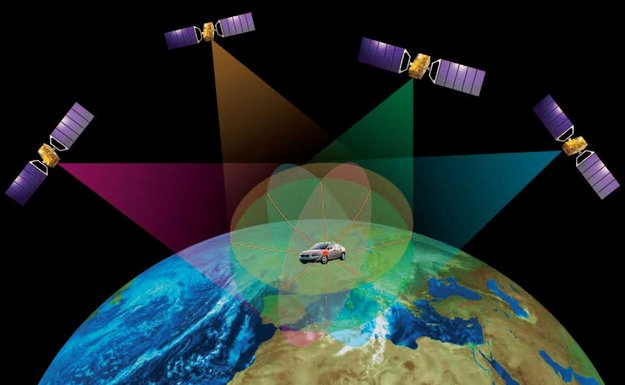
\includegraphics[width=0.4\textwidth]{pictureNav}
		\caption{Satellite navigation~\cite{bookProcessing} }
		\label{Fig:nn}
		
	\end{figure}
	The Global Navigation Satellite System term refers to the constellation of satellites broadcasting ranging signals and Navigation Messages (NM). By definition, the GNSS has a global coverage.
	
	
	Nowdays, there are several GNSSs.
	The US-operated Global Positioning System (GPS) is most commonly used
	in commercial applications. GPS is owned by US Government and operated by US Air Force. It provides two levels of operability. While one is restricted to authorised (often military) users, the other is free of charge for everyone with the GPS-capable receiver.
	The second one is Russia Global'naya Navigatsionnaya Sputnikovaya Sistema (GLONASS).
	The third is Galileo, owned and operated by European Union and scheduled to become full operable by 2020 ~\cite{bookProcessing}.
	China is in process of expanding its regional BeiDou Navigation Satellite System into global one by 2020 ~\cite{bookProcessing}.
	In remaining sections, we will concentrate on the GPS system.
	
	\subsection{Navigation Message}\label{sec:NM}
	Each satellite provides data required for utilisation of the positioning determination process in a form of Navigation Message (NM). Figure \ref{Fig:aaa}
	shows the overview of content and structure of the satellite navigation message ~\cite{GPS:1}.
	
	\begin{figure}[H]
		\centering
		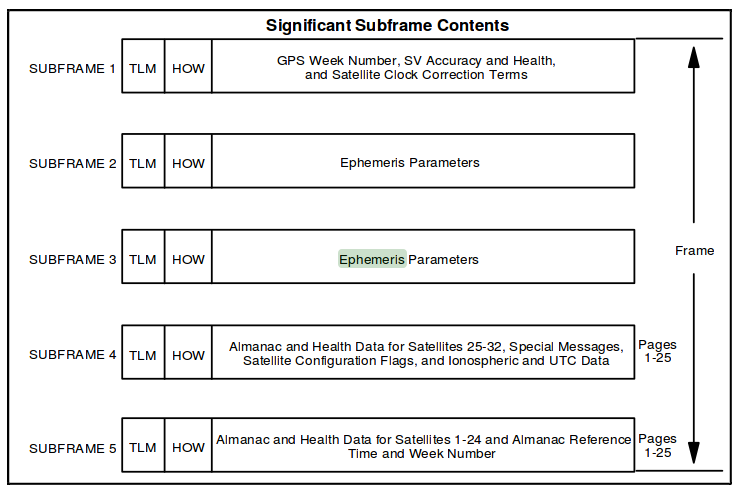
\includegraphics[width=0.4\textwidth]{NACONTENT}
		\caption{Navigation Message Content and Format Overview - one frame \cite{GPS:1}}
		\label{Fig:aaa}
	\end{figure}
	
	A navigation message consists of 25 frames~\cite{bookProcessing}.
	One frame contains 5 sub-frames.
	Each frame contains information about the satellite system time when the next frame is transmitted. 
	Each sub-frame needs 6 seconds to be transmitted.
	The receiver is potentially capable of getting a new pseudo-range at the beginning of each sub-frame, or every 6 
	seconds. 
	%The term message will be reference to one sub-frame, as one sub-frame is efficient to calculate pseudo-range.
	The pseudo-range is indirectly measured distance from transmitting satellite to the receiver.
	
	For the purposes of the discussion, it is sufficient to understand that each navigation message is a set of 
	%signals - this usually refers to the PRN sequences
	binary data where each contains positioning and timing data (sending time, sender-satellite orbit, "satellite ID").
	\begin{figure}[H]
		\centering
		
\includegraphics[width=0.4\textwidth]{message}
		\caption{Navigation Message simplified}
		\label{Fig:na}
	\end{figure}
	
	A detailed description of GPS and GLONASS Navigation Message and the positioning determination algorithm can be found in  ~\cite{bookProcessing}. The same source contains detailed description of positioning determination process. General approach is described in next subsection.
	
	\subsection{Position determination process}\label{sec:positionProcess}
	To determine receiver position, the latitude, longitude and altitude need to be determined. Having 3 unknown parameters, there is need for at least 3, actually 4 (explained later), lineary independent equations.
	
	The orbital data allows the receiver to calculate satellite position in 
	Earth-Centered, Earth-Fixed $\mathnormal{X}$, $\mathnormal{Y}$, $\mathnormal{Z}$ (ECEF XYZ) coordinates.~\cite{GPS:overview}
	\begin{figure}[H]
		\centering
		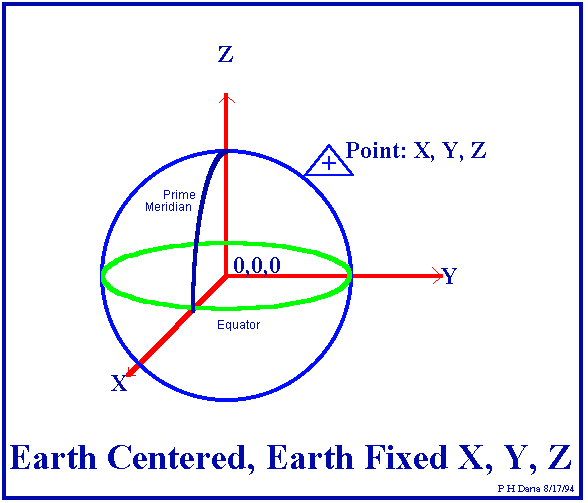
\includegraphics[width=0.4\textwidth]{ecefxyz.png}
		\caption{Earth-Centered, Earth-Fixed $\mathnormal{X}$, $\mathnormal{Y}$, $\mathnormal{Z}$  (ECEF XYZ) coordinates~\cite{GPS:overview}}
		\label{Fig:na}
	\end{figure}
	
	Each receiver has a clock which enables calculation of the signal, navigation message, received time $t'$.
	Let denote the "sending time" of the message of $i$-th satellite with $t_i$.
	Message travelling time is computed as 
	$(t'_i-t_i)$\footnote{
		More precise, travelling time is actually calculated by aligning pseudocode sequences
		(PRN codes).  Both the satellite and GPS receiver generate the same pseudocode at the same time. The satellite transmits the pseudocode which is received by the GPS receiver. 
		The receiver is still producing the pseudocode while the satellite's code is travelling. Eventually, the 2 signals are compared. The difference between the 2 signals is the travel time.}
	
	The receiver-satellite pseudo-ranges are defined as follows:
	$$d_i = c\times(t'_i-t_i)$$
	
	The assumption that satellite signals travel at the speed of light, approximately 300 000 km per second, as they do in vacuum, can be made.
	
	%Correct determination requires or the receiver time/clock to be synchronized with the satellite system time/clock as the forth unknown $d_t$.
	The satellite positioning process requires the perfect syncronisation of the receiver's clock with the common GPS system time (UTC). However, the receiver's clock is usually a quarz electronic clock
	with the time syncronisation error of approximately $10^{-6}$ s (equivalent to approximately 300m pseudo-range error) due to requirements for affordable price of user equipment. Still, the 
	significant user clock error remains the same for all the pseudo-range measurments and regardless of the satellite. This makes the user clock error the forth unknown that describes the user's state , along with three unknown coordinates of positioning.
	
	The pseudo-ranges equation is then following:
	$$d_i = c\times(t'_i- t_i+ d_t)$$
	
	\bigbreak
	Let  $\mathnormal{(x_i, y_i, z_i), i \in \{1,2,3,4\}}$ be the positions of 4 different satellites and $(\mathnormal{x}, \mathnormal{y}, \mathnormal{z})$ the unknown receiver position expressed in ECEF coordinates.
	
	The following (positioning estimation) equations in respect to $\mathnormal{x, y, z}$ and $d_t$ need to be solved:
	
	$$ d_1 = c\times(t'_1- t_1+ d_t) = \sqrt{(x-x_1)^{2}+(y-y_1)^{2}+(z-z_1)^{2}} $$
	$$ d_2 = c\times(t'_2- t_2+ d_t) = \sqrt{(x-x_2)^{2}+(y-y_2)^{2}+(z-z_2)^{2}} $$
	$$ d_3 = c\times(t'_3- t_3+ d_t) = \sqrt{(x-x_3)^{2}+(y-y_3)^{2}+(z-z_3)^{2}} $$
	$$ d_4 = c\times(t'_4- t_4+ d_t) = \sqrt{(x-x_4)^{2}+(y-y_4)^{2}+(z-z_4)^{2}} $$
	
	As we can observe, at least 4 visible satellites need to be visible \footnote{In practice, even larger number of satellites is used to improve the accuracy of positioning determination process.}.
	Visible satellite $\mathnormal{S}$ by the receiver $\mathnormal{R}$ at the time $\mathnormal{T}$ is every satellite from which $\mathnormal{R}$, at the time $\mathnormal{T}$, measures the signal propagation time (i.e., determine the pseudo-range) and derives the positioning estimation equation.
	
	Each receiver is able to transform ECEF coordinates into geodetic latitude, longitude and altitude.

\chapter[Algoritam procjene položaja u domeni navigacijske primjene][Procjena položaja]{Algoritam procjene položaja u domeni navigacijske primjene}
\section[Naslov sekcije u sadržaju][Kratki naslov sekcije]{Osnovni algoritma}
\section[Naslov sekcije u sadržaju][Kratki naslov sekcije]{Izvedba algoritma i procjena točnosti}
Kratki opis koraka koje smo napravili prilikom izvedbe.
\subsection{Zahtjevi algoritma}
Ulaz (U rinex) + uzorak za usporedbu(RINEX)
\subsubsection{RINEX}
-objašnjenje pojma + primjeri. + otkuda nam.
\subsubsection{Programski određen GPS prijemnik}
+zašto i kako smo ga koristili. i dobili podatke. (User manual?)

\subsection{Izvedba}
R kod
\subsection{Procjena točnosti}
+uočene pogreške, uvjetovanost matrice.
\section[Naslov sekcije u sadržaju][Kratki naslov sekcije]{Poboljšani algoritam i njegova izvedba}
Zašto , kako smo došli do toga!
\subsection{Izvedba}
R kod
\subsection{Procjena točnosti}
kako već

\section[Naslov sekcije u sadržaju][Kratki naslov sekcije]{Usporedba osnovnog i poboljšanog algoritma} + zaključak zašto je bolji.

\section[Naslov poglavlja u sadržaju][Kratki naslov poglavlja]{Zaključak}


%\label{stranica}
%Na stranici \pageref{stranica} se nalaza slika u \textbf{png} formatu.

\bibliographystyle{babamspl} % babamspl ili babplain

% U datoteku diplomski.bib se stavljaju bibliografske reference
% Bibliografske reference u bib formatu se mogu dobiti iz MathSciNet baze, Google Scholara, ArXiva, ...
\bibliography{diplomski}

\pagestyle{empty} % ne zelimo brojanje sljedecih stranica

% I na koncu idu sazeci na hrvatskom i engleskom

\begin{sazetak}
Ukratko ...
\end{sazetak}

\begin{summary}
In this ...
\end{summary}

% te zivotopis

\begin{cv}
Dana ...
\end{cv}

\end{document}